\documentclass[11pt]{article}

\usepackage{graphicx}
\usepackage{amsmath}
\usepackage{amssymb}
\usepackage{enumerate}
\usepackage{verbatim}
\usepackage{url}
\usepackage{listings}
\usepackage{float}
\usepackage{color}
\usepackage{subfig}
\usepackage{biblatex}
\usepackage{hyperref}
\usepackage{filecontents}
%%%%%%%%%%%%%%%%%%%%%%%%%%%%%%
\oddsidemargin  0.0in
\evensidemargin 0.0in
\textwidth      6.5in
\headheight     0.0in
\topmargin      0.0in
\textheight     9.0in

\definecolor{mygreen}{RGB}{28,172,0} 
\definecolor{mylilas}{RGB}{170,55,241}
%%%%%%%%%%%%%%%%%%%%%%%%%%%%%%


%%%%%%%%%%%%%%%%%%%%%%%%%%%%%%
\begin{document}

\lstset{language=Matlab,%
    %basicstyle=\color{red},
    breaklines=true,%
    morekeywords={matlab2tikz},
    keywordstyle=\color{blue},%
    morekeywords=[2]{1}, keywordstyle=[2]{\color{black}},
    identifierstyle=\color{black},%
    stringstyle=\color{mylilas},
    commentstyle=\color{mygreen},%
    showstringspaces=false,%without this there will be a symbol in the places where there is a space
    numbers=left,%
    numberstyle={\tiny \color{black}},% size of the numbers
    numbersep=9pt, % this defines how far the numbers are from the text
    emph=[1]{for,end,break},emphstyle=[1]\color{red}, %some words to emphasise
    %emph=[2]{word1,word2}, emphstyle=[2]{style},    
}

\title{Problem Solving by Computer: Coursework 2}      % put your title here
\author{Struan McDonough UID: 8933639}      % name and UID
\date{\today}
\maketitle

\section{Formulating the Problem}

\subsection{The setup}
In the given scenario, one can identify three important components: the scene, the configuration, and the moving entities.

The scene is simple: it contains information about where the fox and the rabbit start, and a position the rabbit moves towards. The scene also contains a warehouse, made of a north, south and west wall, which cannot be seen or passed through by either animal.

Finally, the animals each have their own set of rules. The rabbit will always move towards its burrow. The fox will always move towards the rabbit, as long as there is a line of sight between it and the rabbit. If there is no line of sight, the fox will move towards the corner where the rabbit was last seen.

\subsection{The movement}
The most challenging aspect I encountered while modelling this scenario is describing how the fox moves. In contrast, the rabbit follows a linear path, and its position can be described over time using Euclidean distance.

The fox's position is dependent on the position of the rabbit, so the rabbit's position must be calculated first. One also needs to be able to determine if a line of sight exists between the fox and the rabbit. Once we have determined what position the fox will traverse towards, we can use the same Euclidean process used by the rabbit, to direct the fox to its next position.

\subsection{The decay}
In the second scenario, both the rabbit and the fox experience an exponential decay in their speed. The decay is proportional to the distance travelled. This means that one must hold the distance travelled for each animal at any given time point, in order to calculate the adjusted speed.

\section{Solving the Problem}

\subsection{Main Logic}

The main logic for the solution is described in the \textit{FoxChase.m} function. This function takes two parameters:

\begin{enumerate}
	\item A float representing the time between each simulation sample.
	\item A boolean representing whether the simulation should take into account the exponential decay.
\end{enumerate}

The approach I took to the simulation was to first initialise the information for the main components identified in the problem's formulation: the scene, the configuration and the moving entities. To this end, I packaged the required constants and expected variables into structs representing each of these components. I was careful to name any constants in \textit{UPPER\_CASE} and any variables in \textit{PascalCase}. This makes it clear during programming that the constants should never be updated.

I then initialised the scene's current time to 0, and then repeated the following process for each time increment, until one of the termination conditions had been met.

\begin{enumerate}
	\item {Determine the rabbit's current position.}
	\item {Determine the fox's current position.}
	\item {Log the animals' positions to produce a plot later.}
	\item {Determine if a termination condition has been met.}
	\item{Update the current time by the pre-defined time increment.}
\end{enumerate}

To keep the solution modular and organised, I separated the logic for the movement of the animals into their own functions, which are \textit{FoxPosition.m} and \textit{RabbitPosition.m} respectively. 

After this process had completed, I use the logged data to plot the results, which are then displayed to the user. This is achieved by calling the \textit{PlotHistory.m} function and providing it the logged data.

\subsubsection{Implementation}

\begin{lstlisting}
function rabbitCaught = FoxChase(timeIncrement, speedDecay)
  
  scene = struct; % Struct representing the simulation scene
  scene.BURROW        = [600, 600];
  scene.FOX_START     = [250, -550];
  scene.RABBIT_START  = [0, 0];
  scene.WAREHOUSE_NW  = [200, 0];
  scene.WAREHOUSE_NE  = [800, 0]; % Arbitrary X, defines north wall
  scene.WAREHOUSE_SE  = [800, -400]; % Defines south wall
  scene.WAREHOUSE_SW  = [200, -400];
  scene.CurrentTime   = 0;
  scene.RabbitCaught  = false;
  scene.RabbitEscaped = false;
  
  config = struct; % Struct representing abstract configuration
  config.DISTANCE_CATCH = 0.2; % Min distance for fox to catch rabbit
  config.SPEED_DECAY    = speedDecay; % If speed decay is simulated
  config.TIME_INCREMENT = timeIncrement; % Fidelity of the simulation
  
  fox = struct;
  fox.SPEED_DECAY = 0.0002;
  fox.Distance    = 0;
  fox.History     = [];
  fox.Position    = scene.FOX_START;
  fox.Speed       = 16;  
  
  rabbit = struct;
  rabbit.SPEED_DECAY = 0.0007;
  rabbit.Distance    = 0;
  rabbit.History     = [];
  rabbit.Position    = scene.RABBIT_START;
  rabbit.Speed       = 13;
  
  % Continue until a termination condition is met
  while(1)
    
    rabbit = RabbitPosition(rabbit, scene, config); % Update position
    fox = FoxPosition(fox, rabbit, scene, config); % Update position
    
    rabbitRecord = [scene.CurrentTime, rabbit.Position(1), rabbit.Position(2)];
    rabbit.History = [rabbit.History; rabbitRecord]; % Append position to log
    
    foxRecord = [scene.CurrentTime, fox.Position(1), fox.Position(2)]; 
    fox.History = [fox.History; foxRecord]; % Append position to log
    
    % Check if the rabbit has entered its burrow
    rabbitBurrowDistance = EntityDistance(rabbit.Position, scene.BURROW);
    if(rabbitBurrowDistance <= 13 * config.TIME_INCREMENT)
      scene.RabbitEscaped = true;
      disp "The Rabbit escaped...";
      break;
    endif
    
    % Check if the fox had caught the rabbit
    rabbitFoxDistance = EntityDistance(rabbit.Position, fox.Position);
    if(rabbitFoxDistance <= config.DISTANCE_CATCH)
      scene.RabbitCaught = true;
      disp "The Rabbit was caught...";
      break;
    endif
    
    scene.CurrentTime = scene.CurrentTime + config.TIME_INCREMENT;
  endwhile 
  
  % Plot the history and display it to the user
  PlotHistory(fox.History, rabbit.History);
 
\end{lstlisting}

\subsection{Modelling Fox and Rabbit Movements}

\subsubsection{Rabbit Movement}  

The rabbit moves along a linear path and one can determine the distance between the rabbit and its destination. Using this distance, one can then use the rabbit's speed to see what percentage of the total distance the rabbit will travel within one increment of time. Given this percentage of the total distance, one can convert this into a percentage of the total $x$ and $y$ distance, giving the distance the rabbit must travel in both. This distance is then added to the rabbit's current position.

The distance determined is also dependent on whether or not the rabbit is experiencing decay in its speed. If so, we apply the model $s_r(t) = s_{r0}e^{-\mu_rd_r(t)}$, with $s_r$ being the initial speed of the rabbit, $\mu_r$ being the defined decay constant, and $d_r(t)$ being the distance the rabbit has travelled.

\bigskip

\begin{lstlisting}
function [rabbit] = RabbitPosition(rabbit, scene, config)
  
  % Determine the direct distance the rabbit will travel
  differenceX = scene.BURROW(1) - scene.RABBIT_START(1);
  differenceY = scene.BURROW(2) - scene.RABBIT_START(2);
  distanceEuclid = sqrt(differenceX^2 + differenceY^2);
   
  if(config.SPEED_DECAY)
    decayedSpeed = rabbit.Speed * exp(-rabbit.SPEED_DECAY * rabbit.Distance);
    distanceStep = decayedSpeed * config.TIME_INCREMENT;
  else
    distanceStep = rabbit.Speed * config.TIME_INCREMENT;
  endif
  
  percentTravelled = distanceStep / distanceEuclid; 
  rabbit.Distance = rabbit.Distance + distanceStep;

  % Convert this into X and Y distances
  distanceX = percentTravelled * differenceX;
  distanceY = percentTravelled * differenceY;
  
  % Update the Rabbit's position
  positionX = rabbit.Position(1) + distanceX;
  positionY = rabbit.Position(2) + distanceY;
  rabbit.Position = [positionX, positionY];
\end{lstlisting}

\subsubsection{Fox Movement}

The fox moves towards its target using the same model as the rabbit. The fox's model also describes speed decay, should it be required by the simulation. The fox's model augments the rabbit model by checking if there exists a line of sight between the two entities using the \textit{LineOfSight.m} function. This then determines the position \textit{traverseTowards}, which the fox will then move towards. \textit{traverseTowards} will indicate the rabbit's position or the applicable corner's position.

\bigskip

\begin{lstlisting}
function [fox] = FoxPosition(fox, rabbit, scene, config)
                                           
  % Set up the scene based on function parameters
  traverseTowards = rabbit.Position;
  
  if(!LineOfSight(fox.Position, rabbit.Position, scene))
    % Rabbit is not visible, run to next corner
    if(fox.Position(2) < scene.WAREHOUSE_NW(2)) % Visited? NW Corner
      traverseTowards = scene.WAREHOUSE_NW;
    endif
    if(fox.Position(2) < scene.WAREHOUSE_SW(2)) % Cascade, SW corner
      traverseTowards = scene.WAREHOUSE_SW;
    endif  
  endif
 
  % Determine the distance the fox needs to travel 
  differenceX = traverseTowards(1) - fox.Position(1);
  differenceY = traverseTowards(2) - fox.Position(2);
  distanceEuclid = sqrt(differenceX^2 + differenceY^2);
  
  % Determine exponential decay factors
  if(config.SPEED_DECAY)
    decayedSpeed = fox.Speed * exp(-fox.SPEED_DECAY * fox.Distance);
    distanceStep = decayedSpeed * config.TIME_INCREMENT;
  else
    distanceStep = fox.Speed * config.TIME_INCREMENT;
  endif
  
  percentTravelled = distanceStep / distanceEuclid; 
  fox.Distance = fox.Distance + distanceStep;
  
  % Convert the direct distance into X and Y distances
  distanceX = percentTravelled * differenceX;
  distanceY = percentTravelled * differenceY;
  
  % Update the fox's position
  positionX = fox.Position(1) + distanceX;
  positionY = fox.Position(2) + distanceY;
  fox.Position = [positionX, positionY];
\end{lstlisting}

\subsection{Utility Functions}

\subsubsection{Line of Sight}
The fox will traverse towards the rabbit, or the next corner, depending on if the rabbit is visible to it. To determine this, one must check if the line between the fox and rabbit's position intersects any of the three warehouse walls presented in the scene. As soon as an intersection is detected, the program does not execute this function further, saving computation. To detect if the lines intersect, the function makes use of \textit{IntersectingLines.m} function.

\begin{lstlisting}
function visible = LineOfSight(entity1, entity2, scene)

  if(LinesIntersect(scene.WAREHOUSE_SW, scene.WAREHOUSE_SE, entity1, entity2))
    visible = false; % South wall is between the entities
    return;
  endif
 
  if(LinesIntersect(scene.WAREHOUSE_SW, scene.WAREHOUSE_NW, entity1, entity2))
    visible = false; % West wall is between the entities
    return;
  endif
  
  if(LinesIntersect(scene.WAREHOUSE_NW, scene.WAREHOUSE_NE, entity1, entity2))
    visible = false; % North wall is between the entities
    return;
  endif
  
  visible = true; % No walls between entities
\end{lstlisting}

\subsubsection{Intersecting Lines}
To determine if two lines intersect, I use an algorithm presented in Andre LeMothe's "Tricks of the Windows Game Programming Gurus" \cite{1}. It begins by observing that if we have two lines $(\textbf{x}, \textbf{x}+\textbf{r})$ and $(\textbf{y}, \textbf{y}+\textbf{s})$, then the two lines intersect if one can find scalars $t, u$ such that $\textbf{x} + t\textbf{r} = \textbf{y} + u\textbf{s} $. This approach would then use Cramer's Rule to solve the equations to find the exact point of intersection(omitted).

\begin{lstlisting}
function intersection = LinesIntersect(point1, point2, point3, point4)
  
  lineP12DistanceX = point2(1) - point1(1);
  lineP12DistanceY = point2(2) - point1(2);
  lineP34DistanceX = point4(1) - point3(1);
  lineP34DistanceY = point4(2) - point3(2);
  
  denominator = (lineP12DistanceX * lineP34DistanceY) - ...
                (lineP34DistanceX * lineP12DistanceY);
  positiveDenominator = false;
  
  if(denominator == 0)
    intersection = false; % No intersection
    return;
  elseif(denominator > 0)
    positiveDenominator = true;
  endif
  
  lineP13DistanceX = point1(1) - point3(1);
  lineP13DistanceY = point1(2) - point3(2);
  inter1Numerator = (lineP12DistanceX * lineP13DistanceY) - ...
                    (lineP12DistanceY * lineP13DistanceX);
  negativeInter1Numerator = (inter1Numerator < 0);
  
  if(negativeInter1Numerator == positiveDenominator)
    intersection = false; % No intersection
    return;
  endif
  
  inter2Numerator = (lineP34DistanceX * lineP13DistanceY) - ... 
                    (lineP34DistanceY * lineP13DistanceX);
  negativeInter2Numerator = (inter2Numerator < 0);
  
  if(negativeInter2Numerator == positiveDenominator)
    intersection = false; % No intersection
    return;
  endif
  
  check1 = (inter1Numerator > denominator) == positiveDenominator;
  check2 = (inter2Numerator > denominator) == positiveDenominator;
  
  if(check1 || check2)
    intersection = false; % No intersection
    return;
  endif
 
  intersection = true; % Intersection found

\end{lstlisting}

\subsubsection{Entity Distance}

This function is responsible for calculating the distance between the positions of two entities. It achieves this by calculating the Euclidean distance using the $x$ and $y$ distance between the two points, by performing $d = \sqrt{x^2 + y^2}$ where $d$ is the found distance.

\begin{lstlisting}
function distance = EntityDistance(entity1, entity2)
  
  % Simple Eulerian distance between the rabbit and the fox
  distanceX = abs(entity1(1) - entity2(1));
  distanceY = abs(entity1(2) - entity2(2));
  distance = sqrt(distanceX^2 + distanceY^2);

\end{lstlisting}

\subsubsection{Plotting Graphs}

This function is responsible for plotting the historic data for both the rabbit and the fox. The scene's warehouse is also plotted using hard-coded points, as a visual aid. I argue for the use of hard-coded variables here, since the display of the building is not part of the numerical solution, but to help interpret the results.

\begin{lstlisting}
function PlotHistory(rabbitData, foxData)
  
  rabbitX = rabbitData(:,2); % Rabbit Path
  rabbitY = rabbitData(:,3);
  foxX = foxData(:,2); % Fox Path
  foxY = foxData(:,3);
  buildingX = [200, 200, 700, 700, 200]; % Building Plot
  buildingY = [0, -400, -400, 0, 0];
  
  plot(rabbitX, rabbitY, '-o', foxX, foxY, '-o', buildingX, buildingY);
\end{lstlisting}

\section{Results}
\label{sec:results}

\subsection{Constant Speed}

The rabbit escapes, with a distance of \textbf{240.61m} between it and the fox. In total, the rabbit travelled \textbf{848.51m} and the fox travelled \textbf{1044.30m}. The chase lasted for \textbf{65.26} seconds. 

This result was achieved by sampling the locations every \textbf{0.01} seconds.

\subsection{Decaying Speed}

The rabbit escapes, with a distance of \textbf{34.20m} between it and the fox. In total, the rabbit travelled \textbf{848.51m} and the fox travelled \textbf{1254.50m}. The chase lasted for \textbf{89.11} seconds. 

This result was achieved by sampling the locations every \textbf{0.01} seconds.

\begin{figure}[htp]%
    \centering
    \hspace*{-2cm}
    \vspace*{-14cm}
    \subfloat{{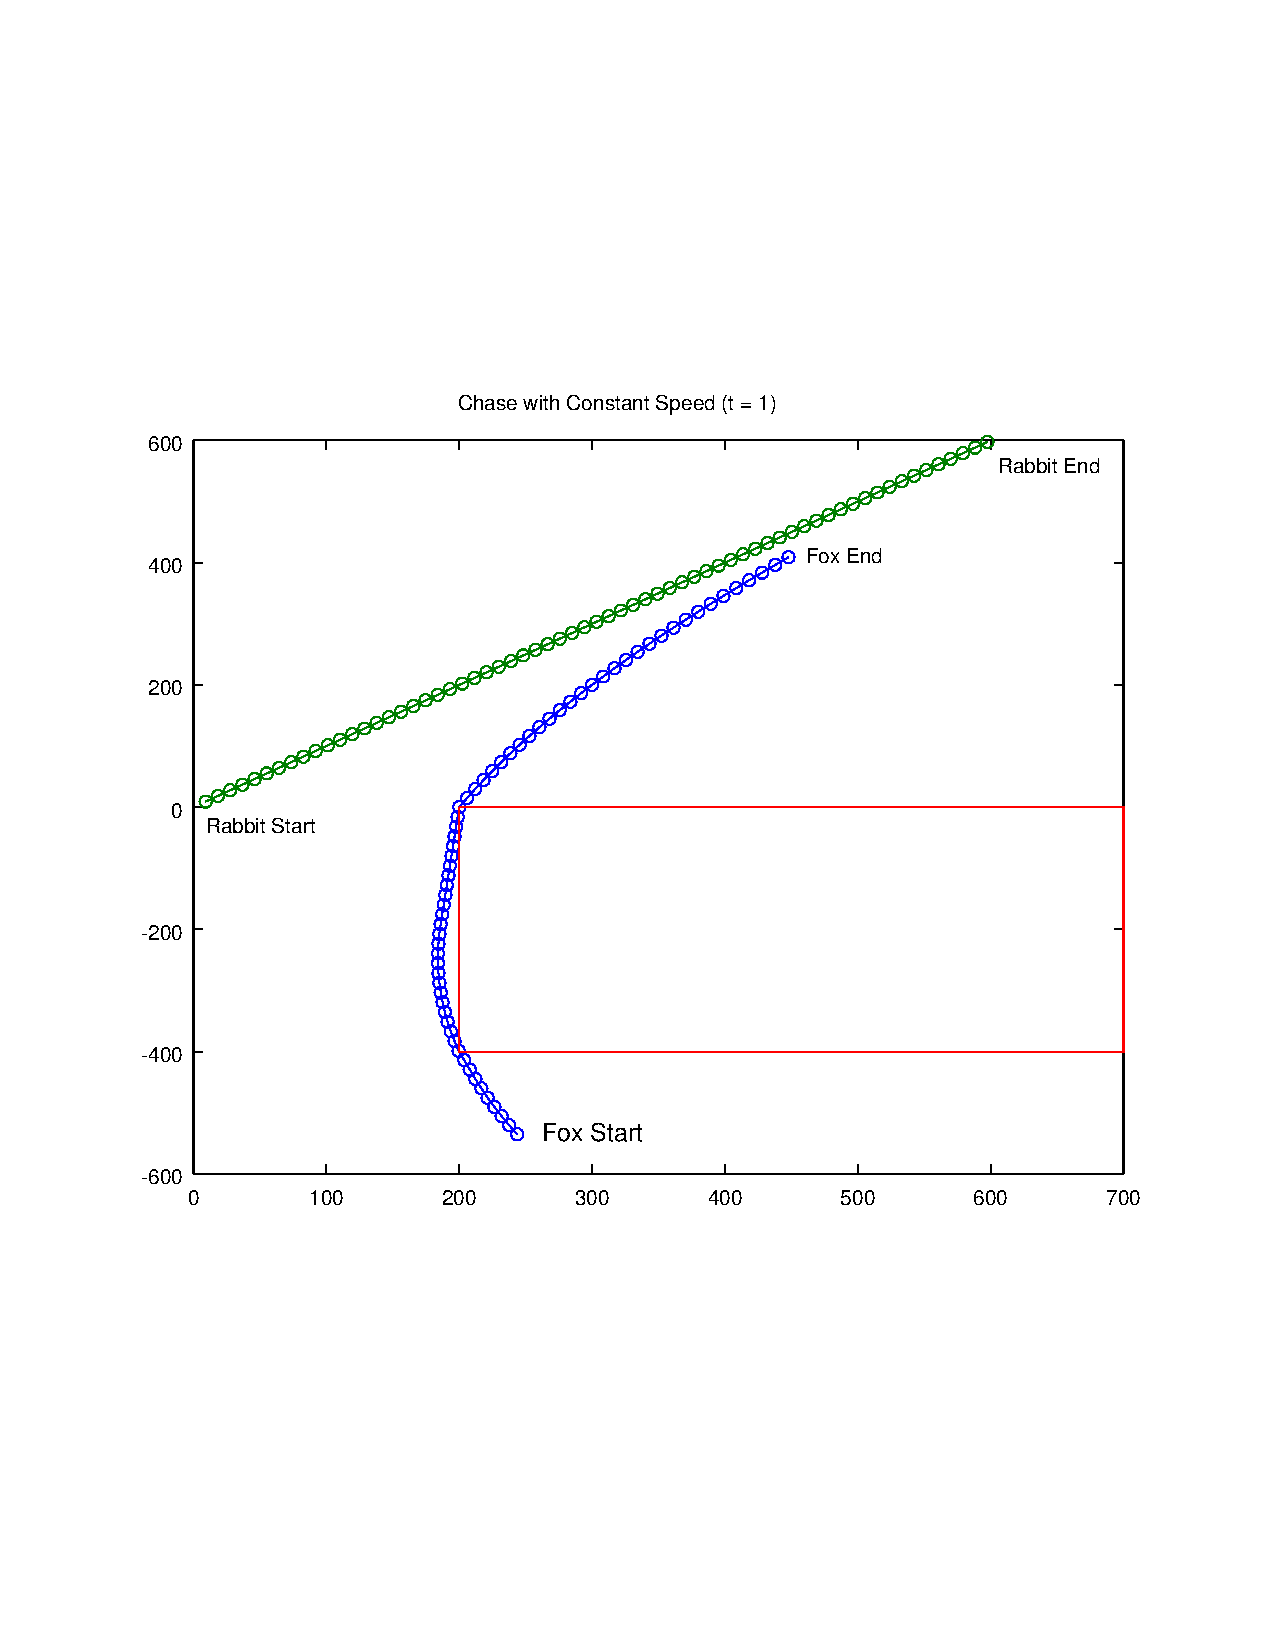
\includegraphics[width=10cm]{no-decay} }}%
    \subfloat{{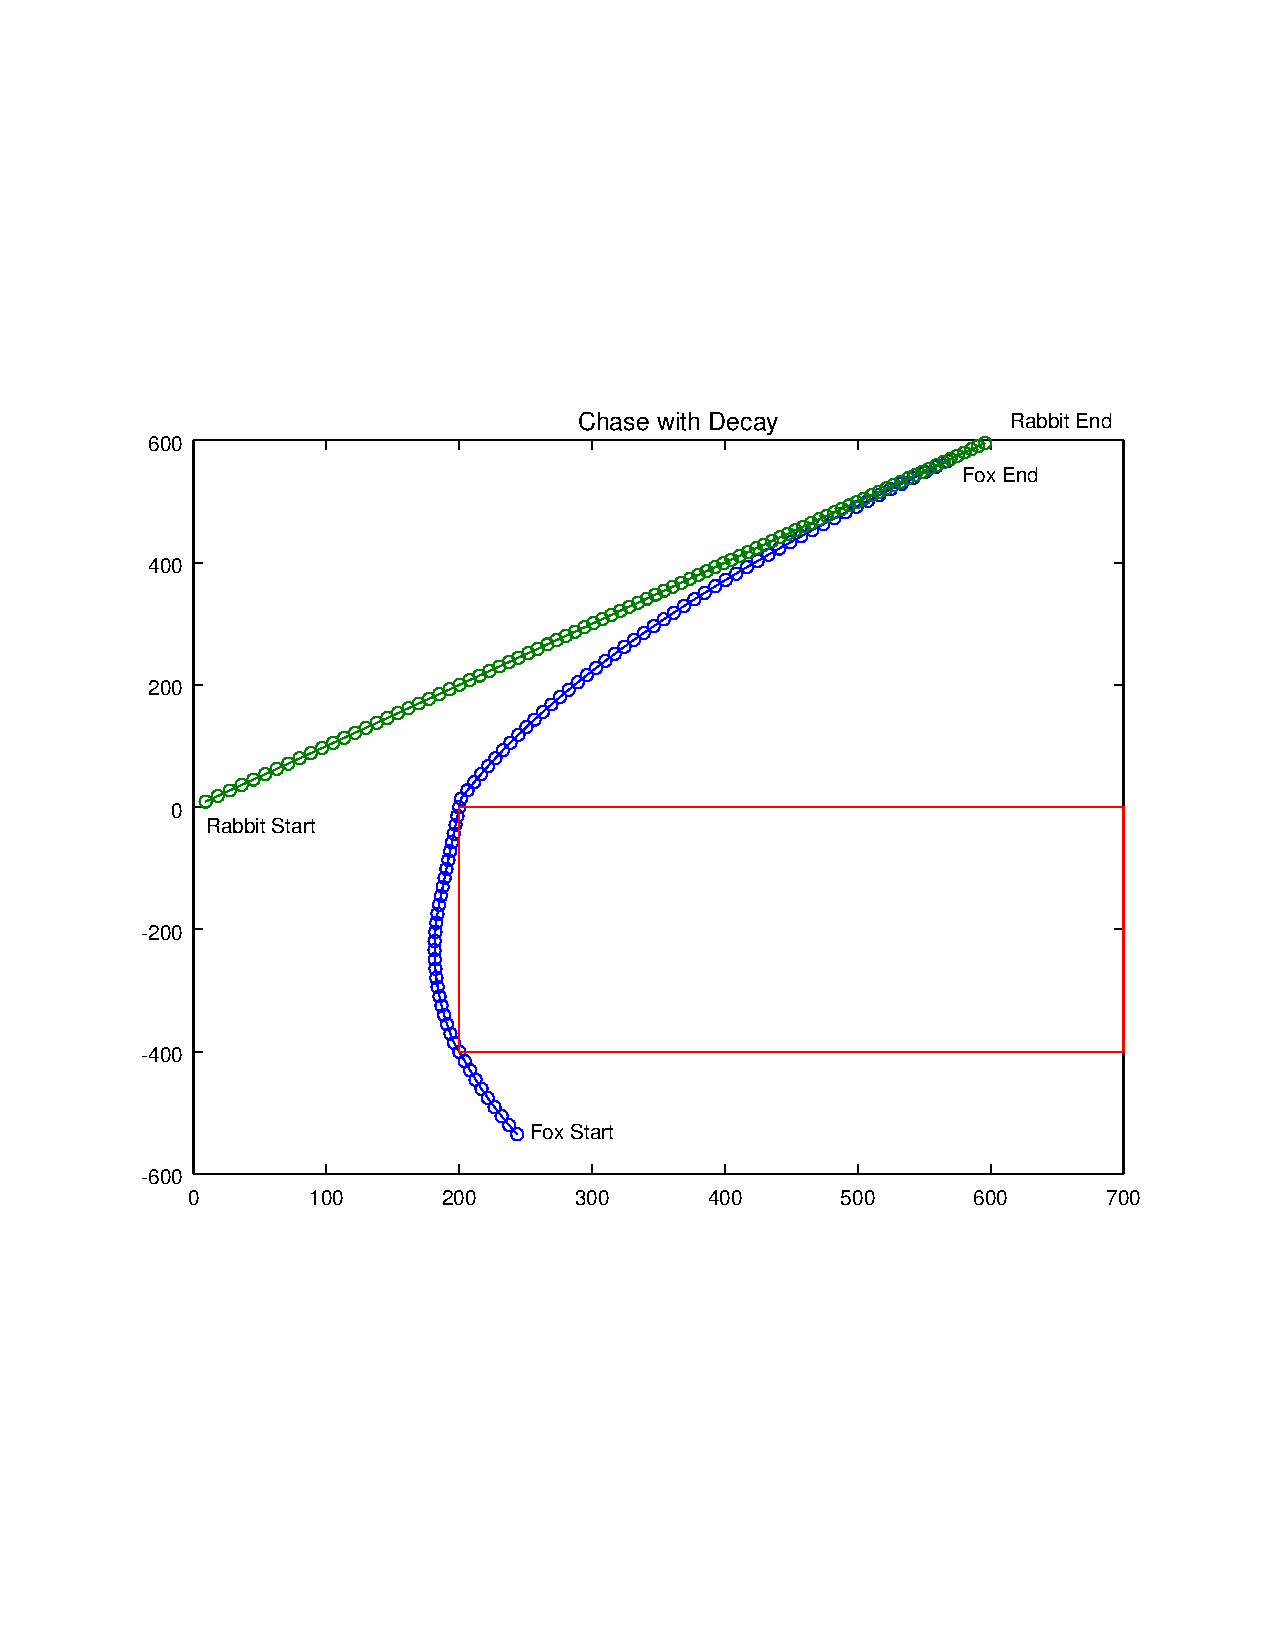
\includegraphics[width=10cm]{decay} }}%
\end{figure}

\begin{thebibliography}{9}

\bibitem{1}
  Andre LaMothe,
  \emph{Tricks of the Windows Game Programming Gurus},
  Sams, Indianapolis,
  2nd edition,
  2002.

\end{thebibliography}

\end{document}